\chapter{Graphics} \label{gnuplot} 
\index{Gnuplot|(}
\index{plotting|see{Gnuplot}}
\index{graphing|see{Gnuplot}}
\index{graphing|see{Graphviz}}

Because graphics formats all have their complexities,
producing graphics from a C program is supremely difficult. You may have
deciphered the correct means of producing JPEGs, but tomorrow you may
need your graph in another format like PDF or PNG or what-have-you.

The solution is to use a handful of external
programs that take in plain text, which is easy to produce by hand or
via C code, and output an image in any of the panoply of graphics
formats.  All of the text-to-graphics programs here are as open and freely
available as gcc, so you can be confident that your code will be portable
to new computers.\footnote{There is some politics about how this is not
strictly true: the maintainers of Gnuplot will not allow you to modify
their code and then distribute the modified package independently (i.e.,
to \airq{fork} the code base). The project is entirely unrelated to the
GNU, and the name is simply a compromise between the names that the two
main authors preferred: nplot and llamaplot.}

The primary coding skill that this chapter covers is programmatically
producing formatted text. You have already been using \ci{printf}-family
functions to display lines of text here and there; this chapter shows
how you can use \ci{printf} functions to produce executable programs.
Appendix A takes a different approach to converting data to an executable
script, via command-line tools to modify text. If your data is not going
through any sort of computations or transformations, you may be better
off using a shell script as per Appendix A instead of writing a C
program as per this chapter.

The plot-producing program with which this chapter will primarily be
concerned is Gnuplot. Its language
basically has only two verbs---\ci{set} and \ci{plot}---plus a few
variants (\ci{splot}, \ci{replot}). Here is a typical Gnuplot script;
you can see that it
consists of a string of \ci{set} commands to indicate what the axes
should look like, the point and line formats, et cetera, and a final
\ci{plot} command to do the actual work.
\begin{lstlisting}
set key off
set xrange [-10:10]
set linewidth 3
set term postscript color
set out 'two_lines.eps'
plot 'datafile' with lines
\end{lstlisting}

\paragraph{Running it}
As with SQLite, there is a command-line interpreter for Gnuplot's
commands (\bi{gnuplot}), so you can
interactively try different \ci{set} commands to see what options look
best. After you have finished shopping for the best settings, you can
put them into a script that will always produce the perfect plot, or
better still, write a C program to autogenerate a script that will
always produce the perfect plot.

The easiest way to put together a script is to put it in a separate file
(e.g., a file named \bi{plotme}) and have Gnuplot read the script. There
are three ways to do this:
\begin{itemize}
\item From the command line, run \bi{gnuplot -persist <plotme}. This runs
the script and exits, but the plot persists on the screen. Without the
\bi{-persist} option, the plot will flash on the screen for a split
second. If you are writing to a Postscript file rather than looking at
the plot on screen, then the \bi{-persist} option is unnecessary.
\item Run \bi{gnuplot} with no options, and from its prompt, type \ci{load
'plotme'}. This leaves you at the Gnuplot prompt to experiment with settings.
\item The hybrid: run \bi{gnuplot plotme -} from the command line. This
executes the instructions in \bi{plotme}, but  leaves you at the Gnuplot
prompt to add settings.
\end{itemize}

If you are at a Gnuplot prompt, you can exit via either the \ci{exit}
command or $<$ctrl$>$-D. On many systems, you can also interact with the plot,
spinning 3-D plots with the mouse or selecting subregions of 2-D plots
to zoom into.

\exercise{Check your Gnuplot installation. Write a one-line text file
named \bi{plotme} whose text reads: \ci{plot sin(x)}. Execute the script
using one of the above methods.}

Now that you know how to run a Gnuplot script, we can move on to what
to put in the script.

\paragraph{Comments} \index{comments!Gnuplot}\index{Gnuplot!comments}
Gnuplot follows the commenting standards of many scripting languages:
everything on a line after a \# is ignored. For example, if a script
begins with
\begin{lstlisting}
#set terminal postscript color
#set out 'printme.eps'
\end{lstlisting}
then these lines are ignored, and Gnuplot will display plots on the
screen as usual. If you later decide to print the plot, you can delete
the \#s and the script will write to \bi{printme.eps}.


\section{\cind{plot}} The \ci{plot} command will set the basic shape of
the plot. 

If you have two columns of data in \bi{datafile}, then to plot a basic
scatterplot of the data, simply specify \ci{plot 'datafile'}. 

You will often dump more columns of data to your datafile than are
necessary. Say that you want to use only the first and fifth columns of
data; then \ci{plot 'datafile' using 1:5}. This produces a scatterplot
with $X$ values from column one and $Y$ values from column $Y$.
Notice that Gnuplot uses index numbering instead of offset numbering:
the first column is one, not zero.

Say that you just want to see a single data series, say column five; then 
\ci{plot 'datafile' using 5}. With only one column given, the plot will
assume that the $X$ values are the ordinal series $1, 2, 3, \dots$ and
your data is the $Y$ values.

\subsection{\cind{splot}} The \ci{plot} command prints flat, 2-D graphs.
To plot 3-D surfaces, use \ci{splot}. All of the above now applies
directly, but with three dimensions. If your data set has three columns, then
you can plot it with \ci{splot 'datafile'}. If your data set has more
than three columns, then specify three with a form like \ci{splot
'datafile' using 1:5:4}. 

\index{surface plots}
Finally, there is the case where the data's  position in the file
represents its position in space, like the ordered series in the 2-D
case. Here, the $(1,1)^{\rm st}$ element in the data file is the
height at the Southwest corner of the plot, and the $(n,n)^{\rm th}$
element is the height at the Northeast corner. To plot such data, use
\ci{splot 'datafile' matrix}.

If all is arranged correctly and you are plotting on-screen instead of
to a file, then you will be able to click on the plot and drag the plot
around its center. The movement vastly improves the 3-D impression of the plot.

Surface plotting goes hand-in-hand with the \cind{pm3d} (palette-mapped
3-D) option, that 
produces a pleasing color-gradient surface. For example, here is the
script used to produce Figure \ref{splotone}. 
\begin{lstlisting}[numbers=left, numberstyle=\scshape, language={}]
set term postscript color;
set out 'plot.eps';
set pm3d;  #for the contour map, use set pm3d map;
unset colorbox
set xlabel 'percent acting'; set ylabel 'value of emulation (n)';
set palette gray;
set xtics ('0' 0,'0.25'  250,'0.5'  500,'0.75'  750, '1' 999);
set ytics ('0' 0, '0.2' 1, '0.4' 2, '0.6' 3, '0.8' 4, '1' 5, '1.2' 6)
splot 'datafile' matrix with pm3d
\end{lstlisting}
Lines one and two send the output to a postscript file instead of the
screen. Line three tells Gnuplot to prepare for a palette-mapped
surface, and is necessary before the \ci{splot} command on line nine.
Line four deletes the legend. 
Line five sets the
labels. Notice that there are two options for ending a Gnuplot command:
you may either put each on a separate line, or put a semicolon between
them. As you can see from this script, ending a line with a semicolon
is optional and harmless.
Line six sets the color scheme to
something appropriate for a book printed in black and white.
There are many palettes to be had; the default, omitting the \ci{set
palette} line entirely, works for most purposes. 
Lines seven and eight fix the axis labels, because Gnuplot defaults to
using the index of the column or row as the label. The format requires a
text label, followed by the index at which the label will be placed.
Producing this by hand is annoying, but it is trivial to write a quick
routine to write such a line:

\begin{lstlisting}
double  n_min           = 0.0;
double  n_max           = 1.4;
double  n_step          = 0.2;

static void deal_with_y_tics(FILE *f){
int  j = 0;
double i;
        fprintf(f, "set ytics (");
        for (i=n_min; i< n_max; i+=n_step){
            fprintf(f, "'%g' %i", i, j++);
            if (i+n_step >=n_max)
                fprintf(f, ")\n");
            else
                fprintf(f, ", ");
        }
}
\end{lstlisting}


Another alternative is to \ci{set pm3d map}. This produces an overhead
view of the same surface, sometimes known as a \vocab{contour plot}, as
in the second plot of Figure \ref{splotone}.

\begin{figure}
\hskip -3.1cm
\begin{tabular}{cc}
\rotatebox{-90}{\scalebox{.36}{\includegraphics{surfaceplot1.eps}}}
&
\rotatebox{-90}{\scalebox{.36}{\includegraphics{surfaceplot2.eps}}}
\end{tabular}
\caption{Two views of the same surface
from a few thousand simulations of a group of agents who decide whether to
act based upon the actions of others. When the coefficient of emulation
is low, the outcomes are unimodally distributed, but outcomes become bimodally
distributed as emulation becomes more desirable.
}\label{splotone}
\end{figure}


\subsection{\cind{replot}} You will often want multiple data sets on the
same plot, and Gnuplot does this easily using the \ci{replot} command.
Just change every use of \ci{plot} after the first to \ci{replot}. 
Page \pageref{replottwo} presents a few more notes on using this
function.

\subsection{Plotting functions} To this point, the discussion has been
entirely about plotting data points, but Gnuplot also knows all of the
functions in the standard C math library. For example, the following
sequence will produce a set of pleasing curves. Notice that \ci{x**2}
is common stats-package notation for $x^2$.  
\begin{lstlisting}
set xrange [-4:6]
plot sin(x)
replot cos(x)
replot log(x) + 2*x - 0.5*x**2
\end{lstlisting}

3-D functions are as effective, e.g.:
\begin{lstlisting}
set pm3d
unset colorbox
splot sin(x) * cos(y) with pm3d
\end{lstlisting}

\section{Some common settings}
At this point, you can produce a basic plot of data or a function (or
both at once). But barring supreme luck, Gnuplot's default plot is not
exactly what you have in mind, and you will need to modify it in some way.

This section catalogs the most common features to set.  
For more information on the settings here and many more, see the
very comprehensive Gnuplot documentation, which can be accessed from
inside the gnuplot command-line program via
\ci{help}, optionally followed by any of the headers below (e.g.,
\ci{help set style}, \ci{help set pointtype}).

Finally, if you are interactively experimenting with settings, bear in
mind that you may have to give a \ci{replot} command (one word with no
options) before the settings take effect.

\subsection{\ci{set style}} The basic style of the plot may be a simple
line or points, a bar plot, boxes with error bars, or many other
possibilities. Gnuplot keeps track of two types of style: that for
function plotting (\ci{set style function}) and for data plotting (\ci{set style data}). 
Thus, a typical style setting would consist of something like \ci{set
style data impulses}.

As with many of Gnuplot's settings, you can either set the style via a
command on its own line, or after the plot command using the \cind{with}
command. There are a few examples below.

\subsection{\ci{set pointtype}, \ci{set linetype}} You can go with the default
point and line type, or explicitly set it using these commands.

Like many Gnuplot commands, they may be given on the same line as the
plot command or on their own line, and may be abbreviated to an
easy-to-type but impossible-to-read two-letter sequence.
\begin{lstlisting}
plot 'data' with points pointtype 3
# is equivalent to
plot 'data' with points pt 3
# is equivalent to
set style data points
set pointtype 3
plot 'data'
\end{lstlisting}

The \ci{pointtype} and \ci{linetype} commands, among a handful of other
commands, may differ from on-screen to postscript
to PNG formats, depending upon what is easy in the different formats.  You can see what each terminal can do via the \ci{test} command. E.g.:
\begin{lstlisting}
set terminal postscript
set out 'testpage.ps'
test
\end{lstlisting}
Among other things, the test page displays the types of points and lines
available for the given terminal, and their number.

\subsection{\ci{set xrange}, \ci{set yrange}} Gnuplot generally does a good job of
selecting a default range for the plot, but you can manually override
this using these commands. A range is of the form \ci{[min:max]}.
Sometimes, you will want to leave one end of the range to be set by
Gnuplot, but fix the other end, in which case you can use a \ci{*} to
indicate an automatically set bound. For example, \ci{set yrange [*:10]}
fixes the top of the plot at ten, but lets the lower end of the plot
fall where it may. 

You will sometimes want the axes to go backward.  Say that your data
represents rankings, so 1 is best; then \ci{set yrange [*:10] reverse}
will put tenth place at the top of the plot, and autoset the bottom of
the plot to just past the largest ranking in the data set.

Ranges may also be put on the plot line. For example:
\begin{lstlisting}
set xrange [-10:10]
set yrange [0:2]
plot 'data'
#is equivalent to
plot 'data' [-10:10][0:2]
\end{lstlisting}

\subsection{\ci{set title}, \ci{set xlabel}, \ci{set ylabel}} These are
very simple commands, that label the $X$
and $Y$ axes and the plot itself. If the plot is going to be a figure
in a paper with an adequate caption, then the title may be optional, but
there is rarely an excuse for omitting axis labels. Sample usage:
\begin{lstlisting}
set xlabel 'Time, days'
set ylabel 'Observed density, picograms/liter'
set title 'Density over time'
\end{lstlisting}

\subsection{\ci{set key}} \index{legend, plot} As noted above, Gnuplot
puts a legend on your plot by default. Most of the time, it is
reasonably intelligent about it, but sometimes the legend gets in the
way. Your first option in this case is to just turn off the key
entirely, via \ci{set key off}.

The more moderate option is to move the key, using some combination of 
\ci{left, right, outside, top, bottom, below}. The first three are
horizontal positions, where \ci{outside} indicates the far right,
outside the plot, while \ci{left} and \ci{right} put the
legend inside the bounds of the plot. The last three indicate vertical
position, where \ci{top} and \ci{bottom} again put the legend inside the
plot, and \ci{below} puts the legend just under the plot.

The key also sometimes benefits from a border, via \ci{set key box}.

For surface plots with \cind{pm3d}, the key is a thermometer displaying
the range of colors and their values. To turn this off, use \ci{unset
colorbox}. See \ci{help set colorbox} on moving or changing the
colorbox's orientation.

\subsection{\ci{set term} and \ci{set out}} \index{Postscript} By 
default, Gnuplot puts a plot on the screen, which is useful for looking
at data, but not necessarily useful for communicating with peers. To
write the plot to a file, you need only select the output file format and name.

Gnuplot's \ci{set terminal} command dictates the language with which to
write the output. \ci{X11} indicates that Gnuplot will be communicating
in the X Window system's terms, \ci{postscript} indicates the Postscript
page display language, \ci{png} indicates the Portable Network Graphics
standard, et cetera. The \ci{set out} command provides a file name to
write to. For example, if a Gnuplot file has 
\begin{lstlisting}
set term postscript color
set out 'a_plot.eps'
\end{lstlisting}
at its head, then the script will not display to the screen and will
instead write the designated Postscript file. See below on further
details on printing.

\subsection{Assorted} Here are a few more settings that you may find
handy.
\begin{lstlisting}
unset border    #Delete the border of the plot.
unset grid      #Make the plot even more minimalist.
set size square  #Set axes to have equal length on screen or paper.
set format y "%.3g" #You can use printf strings to format axis labels.
set format y ""     #Or just turn off printing on the Y axis entirely.
\end{lstlisting}


\section{Printing} \index{Postscript} 
Once your plot looks nice on the screen, you can put it on paper or a
report by simply setting the right variables. Notably, the commands
\begin{lstlisting}
set terminal postscript;
set out 'outfile.eps';
\end{lstlisting}

at the head of a file will put the plot in \bi{outfile.eps} rather
than posting it to the screen. Since all of the plotting commands append
by default, one could start the file off with this command, and then
call a plotting command to produce a paper-printing Gnuplot command file.

The following snippet will erase a file, and
if \ci{print\_to\_paper} is true, place a header setting Gnuplot to
print to \bi{outfile.eps}; if it is false, Gnuplot will default
to printing to screen.

\begin{lstlisting}
char *gnuplot_file = "plot_me";
char *plot_file = "outplot.eps";
FILE    f = fopen(gnuplot_file, "w");//overwrite the file
    if (print_to_paper)
        fprintf(f, "set terminal postscript;\nset out '%s';\n", plot_file);
    fclose(f);
    apop_plot_histogram(data, 1000, gnuplot_file);
\end{lstlisting}

What to do with an \bi{eps} file? For those who just want a quick
printout, your best best is probably to run the command \bi{ps2pdf}
to produce a PDF file, which can be viewed with familiar PDF viewers
such as Acrobat Reader. On a system with GhostScript, the \bi{eps} file
can be viewed and printed directly. Since all of this research will
probably eventually turn into a report or paper, you can also smoothly
include it in \LaTeX{} documents.

\subsection{\treesymbol \LaTeX}\index{Latex@\LaTeX} \index{Tex@\TeX}
You have two options when putting a plot in a \TeX{}ed paper: native
\LaTeX{} and Postscript. 

\paragraph{Native format}
Just as you can set the output device to a screen or a Postscript printer,
you can also send it to a \LaTeX-formatted file. One the plus side, the
fonts will precisely match those in your document, and the resolution is
that of \TeX{} itself (100 times finer than the wavelength of
visible light). On the minus side, some features, such as color, are not
available.

Just as you can dump one C file into another via \ci{\#include}, you can
include the Gnuplot output via the \ci{$\backslash$input} command
\begin{lstlisting}
\documentclass{article}
\usepackage{latexsym}
\begin{document}
...
\begin{figure}
\input outfile.tex
\caption{This figure was autogenerated by a C program.}
\end{figure}
...
\end{document}
\end{lstlisting}

Another very common complaint: the Y-axis label isn't rotated right.
The solution provides a good example of how 
you can insert arbitrary \LaTeX{} code into your Gnuplot code.

First, in the Gnuplot file, you set the label to any set of instructions
that \LaTeX{} can understand. Let $\lambda$ be an arbitrary label:
\begin{lstlisting}
set ylabel '\\rotatebox{90}{Your $\lambda$ here.}'
\end{lstlisting}
Notice the double-backslash. Just as with \ci{printf} (see page
\pageref{printf}), expressions like \ci{$\backslash$n} have special
interpretations, so to print a plain backslash, you will need to double
it to \ci{$\backslash\backslash$}. 

If you are autogenerating this line from C, then you will again need to
double the backslash for each single backslash you will print to the
Gnuplot file. To print the line above to a file, use:
\begin{lstlisting}
fprintf(out, "set ylabel '\\\\rotatebox{90}{Your $\\lambda$ here}'\n ");
\end{lstlisting}

Two final notes to complete the example: \sinline{$\backslash$rotatebox}
is in the \bi{graphicx} package, so it needs to be called in the preamble: 
\begin{lstlisting}
\usepackage{latexsym, graphicx}
\end{lstlisting}
Second, \binline{xdvi} does not currently support rotation, so if you are
viewing via \TeX's native dvi format, the rotation won't happen. Use
either \binline{pdflatex} or \binline{dvips} to view the output as it
will print.

\paragraph{The Postscript route}\index{Postscript|(}
Which brings us to the second option for including a graphic:
Postscript.

Use the \airq{graphicx} package to incorporate the plot. E.g.:
\begin{lstlisting}[language={}]
\documentclass{article}
\usepackage{graphicx}
\begin{document}
...
\begin{figure}
\rotatebox{-90}{\scalebox{.35}{\includegraphics{outfile.eps}}}}
\caption{This figure was autogenerated by a C program.}
\end{figure}
...
\end{document}
\end{lstlisting}
Notice that you will frequently need to rotate the plot $90^\circ$
and scale the figure down to a reasonable size.

The first option for generating PDFs is to use \bi{epstopdf}. First,
convert all of your \bi{eps} files to \bi{pdf} files on the command
line:
\begin{lstlisting}[language=bash]
for i in *.eps; do 
    epstopdf $i;
done
\end{lstlisting}

Then, in your \LaTeX{} header, add 
\begin{lstlisting}[language=sql]
\usepackage[pdftex]{epsfig}
\end{lstlisting}

The benefit to this method is that you can now run \bi{pdflatex
my\_document} without incident; the drawback is that you now have two
versions of every figure cluttering up your directory, and must
regenerate the PDF version of the graphic every time you regenerate the Postscript
version.

The alternative is to go through Postscript in generating the entire
document:
\begin{lstlisting}[language=sql]
latex a_report
dvips < a_report.dvi > a_report.ps
ps2pdf a_report.ps
\end{lstlisting}

This is a lot of typing, but there is a way to automate the process:
\ind{make}. Below is a sample Makefile for producing a \LaTeX{} document
should \bi{pdflatex} be quarrelsome on your system. As with your C
programs, once the Makefile is in place, you can generate final PDF
documents by just typing \bi{make} at the command line. The
creative reader could readily combine this Makefile with the sample C
Makefile from page \pageref{make} to regenerate the final report every
time the analysis is updated.

\begin{lstlisting}[language=make]
DOCNAME = a_report

pdf:	$(DOCNAME).pdf

$(DOCNAME).dvi: $(DOCNAME).tex
	latex $(DOCNAME); latex $(DOCNAME)

$(DOCNAME).ps: $(DOCNAME).dvi
	dvips  -f < $(DOCNAME).dvi > $(DOCNAME).ps

$(DOCNAME).pdf: $(DOCNAME).ps
	ps2pdf $(DOCNAME).ps  $(DOCNAME).pdf

clean:
	rm -f $(DOCNAME).blg $(DOCNAME).log $(DOCNAME).ps
\end{lstlisting}
\index{Postscript|)}


\section{From arrays to plots} \label{gnuprint}
The scripts above gave a file name from which to read the data (\ci{plot
'datafile'}).  Alternatively, \ci{plot '-'} tells Gnuplot to
plot data to be placed immediately below the \ci{plot} command.

With
the \ci{'-'} trick, the process of turning a matrix into a basic plot is
trivial. Let \ci{data} be an \ci{apop\_data} set whose first and fifth
columns we would like to plot against each other. Then we need to create
a file, put a \ci{plot '-'} command in the first line (perhaps preceded by a series of 
static \ci{set} commands), and then fill the
remainder with the data to be plotted. Below is the basic code to create
a Gnuplot file. Since virtually anything you do with Gnuplot will be a
variant of this code, it will be dissected in detail.  
  \label{fprintf}
\begin{lstlisting}[numbers=left, numberstyle=\scshape]
FILE    *f = fopen("plot_me", "w");
fprintf(f, "plot '-' using 1:5 title 'columns (1,5)'\n");
fclose(f);
apop_matrix_print(data, "plot_me");
\end{lstlisting}

The first option to \cind{fopen} is the file to be written to, and
the second option should be either \ci{"a"} for append or \ci{"w"} for
write anew; in this case, we want to start with a clean file so we use
\ci{"w"}.\footnote{If the argument is \ci{"r"}, you could read from the
file. However, none of the methods in this book involve reading raw text
from a file. See any standard reference on C on the details of opening a
file for reading.} 


As you can see from line two, the syntax for \ci{fprintf} is just like
the syntax for \ci{sprintf}: the first argument indicates to what you
are writing, and the rest is a standard \ci{printf} line, which may
include the usual insertions via \ci{\%f}, \ci{\%i}, and so on.

Since Gnuplot lets us select columns via the \ci{using 1:5} clause, there
is no need to pare down the data set in memory.  Notice again that the
first column in Gnuplot is 1, not 0.

The \ci{title} clause shows that Gnuplot accepts both ``double quotes''
and `single quotes' around text such as file names or labels; since
single quotes are nothing special to C, this makes it much easier to
enter such text.

Line three closes the file, so there is no confusion when, in line four,
we use the standard \ci{apop\_matrix\_print} command to write the data
to the file. We print the matrix instead of the
full \ci{apop\_data} structure so that no names or labels are written.
Since \cind{apop\_data\_print} defaults to appending, the matrix appears
after the \ci{plot} header that we just wrote to the file.
You would need to set \ci{apop\_opts.output\_append = 0} to overwrite.
\cindex{apop\_opts.output\_append}

At the end of this, \ci{plot\_me} will be executable by
Gnuplot, using the forms like 
\ci{gnuplot -persist < plot\_me}, as above.

\treesymbol{} Those experienced with POSIX systems know that a script
can be made executable by itself. The first line of the script must begin
with the special marker \#!, and then give the interpreter that will read
the file, and the script must be given execute permissions. The following
program will produce a self-executing Gnuplot script to plot $\sin(x)$:
\begin{lstlisting}
#include <apophenia/headers.h>
#include <sys/stat.h>
int main(){
    char    filename[]  = "plot_me";
    FILE    *f = fopen(filename, "w");
    fprintf(f, "#!/usr/bin/gnuplot -persist\n\
                plot sin(x)");
    fclose(f);
    chmod(filename, 0755);
    return 0;
}
\end{lstlisting}

\subsection{\treesymbol Instant gratification} \label{popen}
All of the above methods involved writing your commands data to a file and then 
running Gnuplot, but you may want to produce plots as your program runs.
This is often useful for simulations, to give you a hint that all is OK
while the program runs, and to impress your friends and funders. This is
easy to do using a \vocab{pipe}, so named because of UNIX's running
data-as-water metaphor.\footnote{There is a readily available
package named \cind{gnuplot\_i} that provides some functions to simplify
piping commands to Gnuplot. It basically works via the same method as
the one discussed in this section, but has much more code to handle
settings and problem cases.}

The command \cind{popen} does two things: it runs the specified program,
and it produces a data pipe that sends a stream of data produced by your
program to the now-running child program. Any commands you write to the
pipe is read by the child as if someone had typed those commands into
the program directly.

You can write to a pipe just like you would write to a file, using
\cind{fprintf}, meaning that once you have opened the pipe to
Gnuplot, the methods above really do apply directly.

You will want to use \cind{apop\_vector\_print} or
\cind{apop\_matrix\_print} to dump out the actual data. To do so, you
will need to set the output type to \ci{'p'} and specify the output
pipe. Lines 11 through 13 in the sample code below do this.
The command on line 14, \cind{fflush}, ensures that all of the data has
been flushed through the pipe and delivered to Gnuplot.

\label{pipeexample}
\begin{lstlisting}[numbers=left, numberstyle=\scshape]
void plot_vector_now(gsl_vector *data){
static FILE *gp = NULL;
int  i;
    if (!gp)
        gp = popen("/usr/local/bin/gnuplot -persist", "w");
    if (!gp){
        printf("Couldn't open Gnuplot.\n");
        return 0;
    }
    fprintf(gp,"reset; plot '-' \n");
    apop_opts.output_type = 'p';
    apop_opts.output_pipe = gp;
    apop_vector_print(data, NULL);
    fflush(gp);
}
\end{lstlisting} 

The \ci{popen} function takes in the full path to Gnuplot, and a \ci{w}
to indicate that you will be writing to Gnuplot rather than reading from
it. You can find where Gnuplot lives on your machine using the command
\bi{which gnuplot}. The \ci{popen} function then returns a file, here
assigned to \ci{gp}. Since \ci{gp} was declared to be a static function,
and \ci{popen} is only called when \ci{gp==NULL},
it will persist through multiple calls of this function, and you can
repeatedly call the function to produce new plots in the same window.

If \ci{gp} is \ci{NULL} after the call to \ci{popen}, then something
went wrong.  This is worth checking for every time a pipe is created.

But if the pipe was created
properly, then the function continues with the now-familiar process of
writing the command \bi{plot '-'} and a vector to a file. The \bi{reset}
command to Gnuplot ensures that next time you call the function, the new
plot will not have any strange interactions with the last plot.

One final detail: data is often kept in a \vocab{buffer}, a space in
memory that the system promises to eventually write to the file. This
improves efficiency, but you want your plot now, not when the system
deems the buffer worth writing.  The final
function, \cind{fflush}, tells the system to send all elements of the
\ci{gp} buffer down the pipeline. The function also works when you are
expecting standard
output to the screen, by the way, via \ci{fflush(NULL)}.

The main drawback to producing real-time plots is that they can take over
your computer, as another plot pops up and grabs focus every half-second, and can significantly slow down the program.
Thus, you may want to settle for occasional redisplays, such as every
fifty periods of your simulation. You could call the above
function using something like:

\begin{lstlisting}
for (period =0; period< 1000; period++){
    run_simulation();
    if (!(period % 50))
        plot_vector_now(output);
\end{lstlisting}

\exercise{Now would be a good time to plot some data series. At this
point, you should have some data in an \ci{apop\_data} set of some sort.
\begin{itemize}
\item Dump the data to a Gnuplottable file using the above \ci{fprintf}
techniques. 
\item Plot the file, then add \ci{set} commands that you \ci{fprintf} to
file to produce a nicer-looking plot.
\item Modify your program to display the plot immediately using pipes.
How could you have written the program initially to minimize the effort
required to switch between writing to a file and a pipe?
\end{itemize}
}

\subsection{\treesymbol{} \cind{replot} revisited}\label{replottwo}
The \ci{replot} function is a bit fragile to the techniques described
here.

First, it can be very frustrating using the above \ci{plot '-'} format
to put data inline when replotting elements. It is easier to write the
data to a separate file and then refer to that in the file to be read
by Gnuplot. Here is a C snippet to produce a data file and a Gnuplot
command file:
\ns{6}\begin{lstlisting}
FILE    *f = fopen("plot_me", "w");
fprintf(f, "plot 'datafile' using 1 title 'data column 1';\n \
            replot 'datafile' using 5 title 'data column 5';\n");
fclose(f);
apop_data_print(data, "datafile");
\end{lstlisting}
Running \bi{plotme} through Gnuplot will produce a plot with two lines,
representing column one and column five of the datafile.

Also, when outputting to a paper device, replotting tends to make a
mess. Set the output terminal (see below) just before the final replot:
\begin{lstlisting}
plot 'datafile' using 1
set term postscript color
set out 'two_lines.eps'
replot 'datafile' using 5
\end{lstlisting}

\section{Some special plots} For a system that basically only has a 
\ci{set} and a \ci{plot} command, Gnuplot is surprisingly versatile. Here
are some specialized visualizations that go well beyond the basic 2-D
plot.

\subsection{Lattices}  \index{lattices}
Perhaps plotting two pairs of columns at a time is not sufficient---you
want bulk, displaying every variable plotted against every other. For
this, use the \ci{apop\_plot\_lattice} function.

\begin{lstlisting}
apop_data *d = apop_text_to_data("indata", 0, 1);
apop_plot_lattice(d,"outfile");
\end{lstlisting}
This produces a file that (after \bi{gnuplot -persist outfile}) produces
a plot like the one in Figure \ref{trellis}. Each variable is plotted
against each other, so the upper-left plot shows the SES variable
versus the Hirfindahl index for a set of data points. The lower-right
plot shows a mirror image of the same two variables. Along the diagonal
are plots of a variable against itself, and therefore these plots will
always be along the $45^\circ$ line. They give a quick picture of the
how a variable's density is distributed.

\begin{figure}
\rotatebox{-90}{\scalebox{.45}{\includegraphics{trellis.eps}}}
\caption{Three variables from my hard drive. Each is plotted against the
other.}\label{trellis}
\end{figure}

What is a lattice plot good for? Some call it \airq{getting a lay of the
land}, while others call it \vocab{data snooping}. Given ten perfectly
random variables, there is a good chance that at least one pair of
lattice plots will look to you like it demonstrates a nice correlation.
A formal regression on the chosen pair of variables will likely
verify your initial visual impression. 

One interviewer directly asked the people who first developed
this type of display, Rick Becker and Bill Cleveland,
whether this display method treads too close to data
snooping:\footnote{\url{http://stat.bell-labs.com/project/trellis/interview.html}}

\begin{quote}
{\em Interviewer:} OK, but there is another way to approach the study of a large database:
develop a statistical model and see if it fits the data. If it does fit,
use the model to learn about the structure of the data.

{\em Becker \& Cleveland:} Yes, and Trellis
display\footnote{\vocab{Trellis display} is a trademarked term; therefore
this book and many common stats packages use the term \airq{lattice}
to refer to similar displays.} is a big help in doing this because it
allows you to make a good guess about an initial model to fit and then
to diagnose how well it fits the data. [\dots]

{\em Interviewer:} But instead of agonizing over all those panels I could do a bunch of
chi-squared tests for goodness of fit.

{\em Becker \& Cleveland:} You're joking, right? If not, we're leaving.

{\em Interviewer:} OK, I guess I'm joking.
\end{quote}

Since Becker and Cleveland do not elucidate the difference between their
visualization method and numerical data snooping, it is up to you to
decide whether such wide-reaching plots are a good first hack at the
data or merely facilitators of apophenia.

\subsection{Histograms} \index{histograms!plotting|(}\label{histosec}
Gnuplot, refusing to do calculations for you,
makes making histograms a pain.  Fortunately, the GSL has you covered,
with the \cind{gsl\_histogram} object, which will also appear
in Section \ref{randomnumbers}, when we needed to generate PDFs from data.

It creates a set of bins, and
then you can call \ci{gsl\_histogram\_increment} to put
data into the right bin. Below is the code for \cind{apop\_plot\_hist\-o\-gram}. 
It allocates a histogram with
\ci{bin\_ct} bins, then sets its range to just past the min and max
of the data. Then the \ci{for} loop pulls data points from the vector and
dumps them to the histogram, without any further calculation on our part.
Once everything is neatly aggregated, the function opens a file and dumps the data to a Gnuplottable file. There is an example of this function in use in Figure \ref{draw_beta_curve}, page \pageref{draw_beta_curve}.
\begin{lstlisting}
void apop_plot_histogram(gsl_vector *data, size_t bin_ct, char *outfile){
int             i;
FILE *          f;
double          min, max, pt;
gsl_histogram   *h      = gsl_histogram_alloc(bin_ct);
    gsl_vector_minmax(data, &min, &max);
        gsl_histogram_set_ranges_uniform(h, min-GSL_DBL_EPSILON, max+GSL_DBL_EPSILON);
    for (i=0; i < data->size; i++){
        pt  = gsl_vector_get(data, i);
        gsl_histogram_increment(h, pt);
        }

    //Now that you have a histogram, print it.
        if (outfile == NULL)    f       = stdout;
        else            f       = fopen(outfile, "a");
    fprintf(f, "set key off                                     ;\n\
                        set style data histograms               ;\n\
                        set style histogram cluster gap 0       ;\n\
                        set xrange [0:%i]                       ;\n\
                        set style fill solid border -1          ;\n\
                        set boxwidth 0.9                        ;\n\
                        plot '-' using 2:xticlabels(1);\n", bin_ct);
    for (i=0; i < bin_ct; i++)
    fprintf(f, "%4f\t %g\n", h->range[i], gsl_histogram_get(h, i));
    if (outfile !=NULL)    fclose(f);
}
\end{lstlisting}
\index{histograms!plotting|)}

\subsection {Pruning data for display}
Plotting the entire data set may be detrimental for two reasons. The
first is the range problem: that one data point at $Y=$a million throws off the
whole darn plot. If you are using an interactive on-screen plot, you
can select a smaller region, but it would be better to just not plot
that point to begin with. 

The second reason for pruning is when the data set is too large. The black
blob you get from plotting ten million data points on a single piece of
paper is not very informative. In this case, you want to use only a
random subset of the data.

This section forthcoming. Summary: you can do this in SQL using the
typical \sinline{select * from plotme where value < 1e7} form to eliminate
those values greater than a million. 


\summary{
\item A Gnuplot command file basically consists of a group of \ci{set}
commands to specify how the plot will look, and then a single \ci{plot}
(2-D version) or \ci{splot} (3-D version) command. 
\item Using the \ci{plot '-'} form, you can put the data to be plotted
in the command file immediately after the command. You can use this and
\ci{apop\_data\_print} to produce plot files of your data.
}

\section{Animation}\index{animation} Perhaps three dimensions is not
quite enough, and you need one more. Gnuplot easily supports animation:
just stack plots one after the next and call \ci{plot} in between. However,
many media (such as paper) do not yet support animation, meaning that your
output will generally be dependent on your display method. The \ind{GIF} format
provides animation and is supported by all major web browsers, so you
can also put your movies online.\footnote{Also, the U.S. patents on the
compression algorithm upon which the GIF format is based \citep{welch:lzw}
have expired, so the mathematical transformations required to write a
GIF may be executed without seeking a license.}

There are two details that will help you with plotting multiple data
sets. First, Gnuplot reads an \ci{e} alone on a line to indicate the end
of a data set. Second, Gnuplot allows you to define constants via a
simple equals sign. The command \ci{p = 1} creates the variable \ci{p}
and sets it to one. Third, Gnuplot has a \ci{pause n} command that will
wait $n$ seconds before drawing the next plot. 

Tying it all together, say that you have an array of \ci{ct} \ci{apop\_data}
sets. The following function will write a Gnuplottable file to display
them in sequence. Notice that by setting output type to \ci{p}, we don't
need to open and close the output file when switching between
writing with \cind{fprintf} and writing with
\cind{apop\_matrix\_print}.
\begin{lstlisting}
void animate_data_sets(apop_data *d, int ct, char *outfile){
  int   i;
  FILE  *f = fopen(outfile, "w");
    fprintf(f, "set pm3d; \n\
                p = 1;");
    apop_opts.output_type = 'p';
    apop_opts.output_pipe = f;
    for(i=0; i< ct; i++){
        if (i && i< ct-1)
            fprintf(f, "e\n\
                pause p;\n");
        fprintf(f, "splot '-' with pm3d\n");
        apop_matrix_print(d[i]->matrix, outfile);
    }
}
\end{lstlisting}
This will produce an \bi{outfile} that looks something like this:
\begin{lstlisting}
set pm3d;
  p = 1;
splot '-' with pm3d
{data[0] here}
e
 pause p;
splot '-' with pm3d
{data[1] here}
e
 pause p;
splot '-' with pm3d
{data[2] here}
e
\end{lstlisting}

You can run the resulting output file through the Gnuplot command line
as usual. If a one-second pause is too long or too short, you need only
change the single value of \ci{p} at the head of the file to change the
delay throughout.

You can write the above plots to a paper-oriented output format, in which
case each plot will be on a separate page. You could then page through
them with a screen viewer, or perhaps print them into a flipbook. When writing a
file, set \ci{p=0} in the above, since there is no use delaying between
outputs.

\index{Gnuplot|)}

\index{graphing!nodes}
\index{graphing!flowcharts}
\index{Graphviz|(}
\index{dot, graphing program}
\section{\treesymbol Graphs---nodes and flowcharts} In common conversation, we
typically mean the word \airq{graph} to be a plot of data like every
diagram to this point in the chapter. The mathematician's definition
of \airq{graph}, however, is a set of nodes connected by edges. The
authors of Gnuplot have no interest in such graphs, so the reader is
referred to another package for graphing, named Graphviz. Like
all of the tools in this book, Graphviz installs itself
gracefully via your package manager. If you have network data that you
would like to visualize, this is the package to use.

The package includes various executables, the most notable of which are
\ci{dot} and \ci{neato}. Both take the same input files, but \ci{dot}
produces a flowchart where there is a definite beginning and end, while
\ci{neato} produces more amorphous plots that aim only to group nodes
via the links connecting them. 

The programs are similar to Gnuplot in that they take in a plain text
description of the nodes and edges, and produce an output file in any of
a plethora of graphics formats.  The syntax for the input files is 
entirely different from Gnuplot's, but the concept should be familiar to
you at this point: there are elements to describe what the nodes and
edges should look like, interspersed with data listing which nodes link
to which. 

For example, flip back to page \pageref{modelflowback} and have a look at
Figure \ref{modelflowback}. One would produce this graph using the following
input to \ci{dot}:

\begin{lstlisting}
digraph {
    rankdir = LR;
    node [shape=box];
    "Data" -> "Estimation" -> "Parameters";
}
\end{lstlisting}
The lines with \ci{=} in them set parameters, stating that the
graph should read left-to-right instead of the top-to-bottom
default, and that the nodes should be boxes instead of the default
ellipses. The line with the \ci{->}s defines how the nodes should link,
and already looks like a text version of Figure \ref{modelflowback}.  By running
\begin{lstlisting}
dot -Tpng <graphdata.dot > output.png
\end{lstlisting}
one could produce a graph much like that in Figure \ref{modelflowback},
in the PNG format. There is a more advanced example below.

At this point, you have all the tools you need to autogenerate a graph.
\index{networks!graphing}
For example, say that you have an $n \times n$ grid where a
one in position $(i,j)$ indicates a link between agents $i$ and $j$ and
a zero indicates no link.
Then a simple \ci{for} loop would convert this data into a
\ci{neato}-plottable file:\label{netlisting}
\begin{lstlisting}
void produce_network_graph(apop_data *link_data, char *outfile){
  FILE *g = fopen(outfile, "w");
  int i,j;
    fprintf(g, "digraph{\n");
    for (i=0; i< link_data->matrix->size1; i++)
        for (j=i+1; j< link_data->matrix->size1; j++)//assume a square matrix.
            if (apop_data_get(link_data, i,j))
                fprintf(g, "node%i -> node%i;\n", i,j);
    fprintf(g, "}\n");
    fclose(g);
}
\end{lstlisting}

In the code supplement,\footnote{\samplecodelocation} you will find 
a file named \bi{data-classroom}, which lists the survey results from a
Junior High classroom in LA, in which students listed their five best friends.
The \airq{ego} column is the student writing down the name of his or her
best friend, and the \airq{nominee} column gives the number of the best
friend. Figure \ref{classnet} graphs the classroom, using \ci{neato} and
the following options for the graph:
\label{graphhead}\begin{lstlisting}
digraph{
    node [label="",shape=circle,height=0.12,width=0.12];
    edge [arrowhead=open,arrowsize=.4];
...
    }
\end{lstlisting}

A few patterns are immediately evident: at the right is a group of four students
who form a complete clique, but do not seem very interested in the rest
of the class. The student above the clique was absent the
day of the survey and thus is nominated as a friend but has no
nominations him or herself; similarly for one student at the lower right. There
are two sets of students who are closely linked, at the left and in
the center, probably representing the boys and the girls. There are two
students who nominated themselves as best friends (one at top right and
one at the bottom), and those two students are not very popular.

\begin{figure}
\begin{center}
\scalebox{.9}{\includegraphics{figs/classnet.eps}}
\caption{The social network of a Junior High classroom.} \label{classnet}
\end{center}
\end{figure}


\exercise{\label{classex} Write a program to replicate Figure \ref{classnet}. 
\begin{itemize}
\item Read the \bi{data-classroom} file into an \ci{apop\_data} set,
using either \ci{apop\_text\_to\_db} and a query, or
\ci{apop\_text\_to\_data}. 
\item Open your output file, and write a header as per page
\pageref{graphhead}.
\item Write a single \ci{for} loop to write one line to the output file for
each line in the data set. Base your \ci{fprintf} statement on the one 
from page \pageref{netlisting}.
\item Close the file.
\end{itemize}
(continued)
} \addtocounter{ex}{-1} \exercise{(continued)

Running the program will produce a \bi{neato}-formatted file.
\begin{itemize}
\item From the command line, run \bi{neato -Tps <my\_output > out.eps}.
The output graph should look just like Figure \ref{classnet}.
\item In the \bi{dot} manual (\bi{man dot} from the command line), you
will see that there are many variant programs to produce different
types of graph. What does the classroom look like via \bi{dot},
\bi{circo}, and \bi{twopi}?
\end{itemize}
The exercise on page \pageref{classextwo} will show you another way to
produce the Graphviz-readable output file.
}

 
\paragraph{Internal use}
If you have been sticking to the philosophy of coding via small,
simple functions that call each other, your code will look like a set
of elements linked via function calls---exactly the sort of network for
which Graphviz was written. If you feel that your code files are getting
a bit too complex, you can use Graphviz to get the big picture.

For example, the SQL tables that produced Figure
\ref{trellis} got a little out of hand. There were many input tables,
intermediate tables, and output tables, some of which were weighted
via one method and some via another. To keep track of them all, I made
a quick scan through the source code to list the source data for each
table (listed below), and then \ci{dot} quickly made sense of it all,
in Figure \ref{sqlplot}.  The syntax of the input file is somewhat
self-descriptive, consisting of the usual setting of characteristics
and then the data describing the connections. Notice that dot's syntax
allows C-style comments.

\begin{lstlisting}
digraph tables {
    edge [arrowhead=open];
//Inputs
    node [color=grey, shape=diamond, style=filled];
    {rank=same; "inhome1" "friend3" "weights";}
//Outputs
    node [color=cyan, shape=box];
    {rank=same; "univariate output" "bivariate output";}
//Nodes with standard weights
    node [style=solid, color=magenta, shape=ellipse];
    "pairs_x" "schoolpcts_x" "ratio_r";
//Intermediates & links
    node [style=solid, color=black, shape=ellipse];
    "weights"   -> "schoolpcts_x" 
    "inhome1" -> "schoolpcts_x" -> "oo_x" 
    "pairs_x" -> "oo_x" -> "univariate output"
    "pairs_x" -> "ratio_l" -> "ratio_paired (c)" -> "bivariate output"
    "schoolpcts_x" -> "ratio_r" -> "ratio_paired (unc)" -> "bivariate output"
    "ratio_r" -> "ratio_paired (c)"
    "ratio_l" -> "ratio_paired (unc)"
    "inhome1" -> "pairs_x" 
    "friend3" -> "pairs_x" 
}
\end{lstlisting}

\begin{figure}
\begin{center}
\scalebox{.65}{\includegraphics{sqlplot.eps}}
\caption{The relations among tables in a messy database, as interpreted by
\ci{dot}. Input tables are at the top, and outputs at the bottom.}\label{sqlplot}
\end{center}
\end{figure}

You could also graph the calling relationships among the functions in
your C code---but before you start manually scanning your code, you
should know that there is a program to do this for you. Ask your package
manager for \ci{doxygen}, which
generates documentation via specially-formatted comments in the source
file. If configured correctly, it will use Graphviz to include call
graphs in the documentation.


\comment{
Figure \ref{modelflow} on page \pageref{modelflow} was drawn by
hand, but Figure \ref{models.dot} shows a dot file to produce a similar
graph. 


\lstset{numbers=left, numberstyle=\scshape}
\codefig{models.dot}{The \ci{dot} rendition of Figure \ref{modelflow}.}
\lstset{numbers=none}

; lines three and four set the default shapes for
edges and nodes. Lines five through ten introduce the cast of
characters. Most nodes (the ones in the \ci{main} group) are simply
known by their labels, but notice that the diagram has two nodes named
\ci{data}, so they are named \ci{node0} and \ci{node1} and assigned a
label. Grouping the 
}

\summary{
\item The Graphviz package produces graphs from a list of edges. Such
lists are easy to autogenerate from C.
\item You can also use Graphviz to keep track of relationships among
functions in your code or tables in your database.
}

\index{Graphviz|)}

